\appendix


\chapter{Archivo xml del TUNA corpus}
\section{Archivo}
\label{archivos-xml-tuna}

Este es el texto del archivo s57t4.xml del TUNA corpus.
\begin{verbatim}
<TRIAL CONDITION="-LOC" ID="s57t4">
  <DOMAIN>
    <ENTITY ID="121" IMAGE="fanLeftBlueSmall.gif" TYPE="target">
      <ATTRIBUTE NAME="colour" TYPE="literal" VALUE="blue" />
      <ATTRIBUTE NAME="orientation" TYPE="literal" VALUE="left" />
      <ATTRIBUTE NAME="type" TYPE="literal" VALUE="fan" />
      <ATTRIBUTE NAME="size" TYPE="literal" VALUE="small" />
      <ATTRIBUTE NAME="x-dimension" TYPE="gradable" VALUE="1" />
      <ATTRIBUTE NAME="y-dimension" TYPE="gradable" VALUE="2" />
    </ENTITY>
    <ENTITY ID="122" IMAGE="fanLeftGreenSmall.gif"
    TYPE="distractor">
      <ATTRIBUTE NAME="colour" TYPE="literal" VALUE="green" />
      <ATTRIBUTE NAME="orientation" TYPE="literal" VALUE="left" />
      <ATTRIBUTE NAME="type" TYPE="literal" VALUE="fan" />
      <ATTRIBUTE NAME="size" TYPE="literal" VALUE="small" />
      <ATTRIBUTE NAME="x-dimension" TYPE="gradable" VALUE="3" />
      <ATTRIBUTE NAME="y-dimension" TYPE="gradable" VALUE="3" />
    </ENTITY>
    <ENTITY ID="57" IMAGE="fanLeftBlueLarge.gif" TYPE="distractor">
      <ATTRIBUTE NAME="colour" TYPE="literal" VALUE="blue" />
      <ATTRIBUTE NAME="orientation" TYPE="literal" VALUE="left" />
      <ATTRIBUTE NAME="type" TYPE="literal" VALUE="fan" />
      <ATTRIBUTE NAME="size" TYPE="literal" VALUE="large" />
      <ATTRIBUTE NAME="x-dimension" TYPE="gradable" VALUE="3" />
      <ATTRIBUTE NAME="y-dimension" TYPE="gradable" VALUE="2" />
    </ENTITY>
    <ENTITY ID="52" IMAGE="fanBackRedLarge.gif" TYPE="distractor">
      <ATTRIBUTE NAME="colour" TYPE="literal" VALUE="red" />
      <ATTRIBUTE NAME="orientation" TYPE="literal" VALUE="back" />
      <ATTRIBUTE NAME="type" TYPE="literal" VALUE="fan" />
      <ATTRIBUTE NAME="size" TYPE="literal" VALUE="large" />
      <ATTRIBUTE NAME="x-dimension" TYPE="gradable" VALUE="2" />
      <ATTRIBUTE NAME="y-dimension" TYPE="gradable" VALUE="1" />
    </ENTITY>
    <ENTITY ID="106" IMAGE="sofaLeftGreenSmall.gif"
    TYPE="distractor">
      <ATTRIBUTE NAME="colour" TYPE="literal" VALUE="green" />
      <ATTRIBUTE NAME="orientation" TYPE="literal" VALUE="left" />
      <ATTRIBUTE NAME="type" TYPE="literal" VALUE="sofa" />
      <ATTRIBUTE NAME="size" TYPE="literal" VALUE="small" />
      <ATTRIBUTE NAME="x-dimension" TYPE="gradable" VALUE="2" />
      <ATTRIBUTE NAME="y-dimension" TYPE="gradable" VALUE="3" />
    </ENTITY>
    <ENTITY ID="41" IMAGE="sofaLeftBlueLarge.gif"
    TYPE="distractor">
      <ATTRIBUTE NAME="colour" TYPE="literal" VALUE="blue" />
      <ATTRIBUTE NAME="orientation" TYPE="literal" VALUE="left" />
      <ATTRIBUTE NAME="type" TYPE="literal" VALUE="sofa" />
      <ATTRIBUTE NAME="size" TYPE="literal" VALUE="large" />
      <ATTRIBUTE NAME="x-dimension" TYPE="gradable" VALUE="3" />
      <ATTRIBUTE NAME="y-dimension" TYPE="gradable" VALUE="1" />
    </ENTITY>
    <ENTITY ID="36" IMAGE="sofaBackRedLarge.gif" TYPE="distractor">
      <ATTRIBUTE NAME="colour" TYPE="literal" VALUE="red" />
      <ATTRIBUTE NAME="orientation" TYPE="literal" VALUE="back" />
      <ATTRIBUTE NAME="type" TYPE="literal" VALUE="sofa" />
      <ATTRIBUTE NAME="size" TYPE="literal" VALUE="large" />
      <ATTRIBUTE NAME="x-dimension" TYPE="gradable" VALUE="4" />
      <ATTRIBUTE NAME="y-dimension" TYPE="gradable" VALUE="3" />
    </ENTITY>
  </DOMAIN>
  <WORD-STRING>blue ventilator center left</WORD-STRING>
  <ANNOTATED-WORD-STRING>
    <ATTRIBUTE ID="a1" NAME="colour" VALUE="blue">blue</ATTRIBUTE>
    <ATTRIBUTE ID="a2" NAME="type" VALUE="fan">
    ventilator</ATTRIBUTE>
    <META-ATTRIBUTE NAME="location">
    <ATTRIBUTE ID="a3" NAME="y-dimension"
    VALUE="2" />center</META-ATTRIBUTE>
    <META-ATTRIBUTE NAME="location">
    <ATTRIBUTE ID="a4" NAME="x-dimension"
    VALUE="2" />left</META-ATTRIBUTE>
  </ANNOTATED-WORD-STRING>
  <ATTRIBUTE-SET>
    <ATTRIBUTE ID="a4" NAME="x-dimension" VALUE="2" />
    <ATTRIBUTE ID="a3" NAME="y-dimension" VALUE="2" />
    <ATTRIBUTE ID="a2" NAME="type" VALUE="fan"></ATTRIBUTE>
    <ATTRIBUTE ID="a1" NAME="colour" VALUE="blue"></ATTRIBUTE>
  </ATTRIBUTE-SET>
</TRIAL>
\end{verbatim}


\section{Calculo probabilidad-GATT para el archivo anterior}

Toma un modelo y calcula la prob\_disc de GATT 

Algoritmo\\
\label{algoritmo-GATT}
\begin{verbatim}
import sys

f=open(sys.argv[1],"r")

f2=open("GATT-"+sys.argv[1],"w")

d=dict()

for line in f.readlines():
    if "    <related rel=" in line:
        pal=line.split('"')[1]
        if pal in d.keys(): d[pal]=d[pal]+1
        else: d[pal]=1

for key in d:
    numero=float(1)/float(d[key])
    f2.write(key+"->"+repr(numero)+"\n")

f.close()
f2.close()

Script para ejecutar en todos los archivos

#!/usr/bin/python
from os import *

l=[1, 3, 6 ,8, 10, 12, 13, 15, 18, 20, 23, 25, 27]
for i in l:
    system('python calculaGATT.py modeloFig'+repr(i)+'Gre7-2.xml')


\end{verbatim}




\label{probabilidad-GATT}

orientation-left	0.2\\
x-dimension-1	1.0\\
colour-green	0.5\\
size-small	0.3333333333333333\\
x-dimension-4	1.0\\
type-fan	0.25\\
size-large	0.25\\
x-dimension-3	0.3333333333333333\\
colour-blue	0.3333333333333333\\
type-sofa	0.3333333333333333\\
x-dimension-2	0.5\\
colour-red	0.5\\
orientation-back	0.5\\
y-dimension-1	0.5\\
y-dimension-2	0.5\\
y-dimension-3	0.3333333333333333\\

\chapter{Archivos arff input de WEKA}
\label{archivos-arff-blue}

Para la propiedad 'blue' (solo con datos de entrenamiento)\\

@relation probabilidad-uso\\

@attribute target-tiene numeric {0,1}\\
@attribute loc numeric {0,1}\\
@attribute disc-gatt REAL\\
@attribute prob-uso REAL\\

@data\\
0,0,0.5,0.0\\
0,0,0.5,0.0\\
1,0,0.3333333333333333,1.0\\
0,0,0.0,0.0\\
0,0,0.0,0.0\\
0,0,0.5,0.0\\
0,0,0.5,0.0\\
0,0,0.5,0.0\\
1,0,0.3333333333333333,1.0\\
0,0,0.0,0.0\\
0,0,0.0,0.0\\
0,1,0.5,0.0\\
1,1,0.3333333333333333,0.0\\
1,1,0.3333333333333333,0.0\\
0,1,0.0,0.0\\
0,1,0.0,0.0\\
0,0,0.5,0.0\\
0,0,0.5,0.0\\
0,0,0.5,0.0\\
1,0,0.3333333333333333,1.0\\
0,0,0.0,0.0\\
0,0,0.0,0.0\\
0,0,0.5,0.0\\
0,0,0.5,0.0\\
0,0,0.5,0.0\\
1,0,0.3333333333333333,1.0\\
1,0,0.3333333333333333,1.0\\
0,0,0.0,0.0\\
0,0,0.5,0.0\\
1,0,0.3333333333333333,1.0\\
1,0,0.3333333333333333,0.0\\
0,0,0.0,0.0\\
0,0,0.5,0.0\\
0,0,0.5,0.0\\
0,0,0.5,0.0\\
1,0,0.3333333333333333,1.0\\
0,0,0.0,0.0\\
0,0,0.0,0.0\\
0,0,0.5,0.0\\
0,0,0.5,0.0\\
0,0,0.5,0.0\\
1,0,0.3333333333333333,1.0\\
1,0,0.3333333333333333,1.0\\
0,0,0.0,0.0\\
0,0,0.5,0.0\\
0,0,0.5,0.0\\
0,0,0.5,0.0\\
1,0,0.3333333333333333,1.0\\
0,0,0.0,0.0\\
0,0,0.0,0.0\\
0,0,0.5,0.0\\
0,0,0.5,0.0\\
0,0,0.5,0.0\\
1,0,0.3333333333333333,1.0\\
0,0,0.0,0.0\\
0,0,0.0,0.0\\
0,0,0.5,0.0\\
0,0,0.5,0.0\\
1,0,0.3333333333333333,1.0\\
1,0,0.3333333333333333,1.0\\
0,0,0.0,0.0\\
0,0,0.0,0.0\\
0,0,0.5,0.0\\
0,0,0.5,0.0\\
0,0,0.5,0.0\\
1,0,0.3333333333333333,1.0\\
1,0,0.3333333333333333,1.0\\
0,0,0.0,0.0\\
0,0,0.0,0.0\\
0,0,0.5,0.0\\
0,0,0.5,0.0\\
1,0,0.3333333333333333,1.0\\
1,0,0.3333333333333333,1.0\\
0,0,0.0,0.0\\
0,0,0.5,0.0\\
0,0,0.5,0.0\\
0,0,0.5,0.0\\
1,0,0.3333333333333333,1.0\\
1,0,0.3333333333333333,1.0\\
0,0,0.0,0.0\\
0,0,0.0,0.0\\
0,1,0.5,0.0\\
0,1,0.5,0.0\\
1,1,0.3333333333333333,1.0\\
0,1,0.0,0.0\\
0,1,0.0,0.0\\
0,0,0.5,0.0\\
0,0,0.5,0.0\\
1,0,0.3333333333333333,1.0\\
1,0,0.3333333333333333,1.0\\
0,0,0.0,0.0\\
0,0,0.0,0.0\\
0,1,0.5,0.0\\
0,1,0.5,0.0\\
1,1,0.3333333333333333,0.0\\
0,1,0.0,0.0\\
0,1,0.0,0.0\\
0,1,0.5,0.0\\
0,1,0.5,0.0\\
0,1,0.5,0.0\\
1,1,0.3333333333333333,1.0\\
1,1,0.3333333333333333,1.0\\
0,1,0.0,0.0\\
0,1,0.0,0.0\\
0,1,0.5,0.0\\
0,1,0.5,0.0\\
0,1,0.5,0.0\\
1,1,0.3333333333333333,1.0\\
1,1,0.3333333333333333,1.0\\
0,1,0.0,0.0\\
0,0,0.5,0.0\\
0,0,0.5,0.0\\
0,0,0.5,0.0\\
1,0,0.3333333333333333,1.0\\
0,0,0.0,0.0\\
0,1,0.5,0.0\\
0,1,0.5,0.0\\
0,1,0.5,0.0\\
1,1,0.3333333333333333,1.0\\
0,1,0.0,0.0\\
0,1,0.0,0.0\\
0,1,0.5,0.0\\
0,1,0.5,0.0\\
0,1,0.5,0.0\\
1,1,0.3333333333333333,1.0\\
0,1,0.0,0.0\\
0,1,0.0,0.0\\
0,1,0.5,0.0\\
0,1,0.5,0.0\\
1,1,0.3333333333333333,1.0\\
1,1,0.3333333333333333,1.0\\
0,0,0.5,0.0\\
0,0,0.5,0.0\\
0,0,0.5,0.0\\
1,0,0.3333333333333333,1.0\\
1,0,0.3333333333333333,1.0\\
0,0,0.0,0.0\\
0,0,0.0,0.0\\
0,1,0.5,0.0\\
0,1,0.5,0.0\\
0,1,0.5,0.0\\
0,1,0.0,0.0\\
0,1,0.0,0.0\\
1,1,0.3333333333333333,1.0\\
1,1,0.3333333333333333,1.0\\
0,1,0.0,0.0\\
0,1,0.0,0.0\\
0,1,0.5,0.0\\
0,1,0.5,0.0\\
0,1,0.5,0.0\\
1,1,0.3333333333333333,1.0\\
0,1,0.0,0.0\\
0,1,0.0,0.0\\
0,1,0.5,0.0\\
0,1,0.5,0.0\\
0,1,0.5,0.0\\
1,1,0.3333333333333333,1.0\\
1,1,0.3333333333333333,1.0\\
0,1,0.0,0.0\\
0,1,0.0,0.0\\
0,1,0.5,0.0\\
0,1,0.5,0.0\\
1,1,0.3333333333333333,1.0\\
0,1,0.0,0.0\\
0,1,0.5,0.0\\
0,1,0.5,0.0\\
0,1,0.5,0.0\\
1,1,0.3333333333333333,1.0\\
1,1,0.3333333333333333,1.0\\
0,1,0.0,0.0\\
0,1,0.0,0.0\\
0,1,0.5,0.0\\
0,1,0.5,0.0\\
1,1,0.3333333333333333,1.0\\
0,1,0.0,0.0\\
0,1,0.5,0.0\\
0,1,0.5,0.0\\
1,1,0.3333333333333333,1.0\\
1,1,0.3333333333333333,0.0\\
0,1,0.0,0.0\\
0,1,0.0,0.0\\
0,1,0.5,0.0\\
0,1,0.5,0.0\\
0,1,0.0,0.0\\
0,1,0.0,0.0\\
0,1,0.5,0.0\\
0,1,0.5,0.0\\
1,1,0.3333333333333333,1.0\\
1,1,0.3333333333333333,1.0\\
0,1,0.0,0.0\\
0,1,0.5,0.0\\
0,1,0.5,0.0\\
1,1,0.3333333333333333,1.0\\
1,1,0.3333333333333333,1.0\\
0,1,0.0,0.0\\
0,1,0.0,0.0\\
0,1,0.5,0.0\\
0,1,0.5,0.0\\
0,1,0.5,0.0\\
1,1,0.3333333333333333,1.0\\
1,1,0.3333333333333333,0.0\\
0,1,0.0,0.0\\
0,1,0.5,0.0\\
1,1,0.3333333333333333,1.0\\
1,1,0.3333333333333333,1.0\\
0,1,0.0,0.0\\
0,1,0.0,0.0\\
0,1,0.5,0.0\\
0,1,0.5,0.0\\
1,1,0.3333333333333333,1.0\\
0,1,0.0,0.0\\
0,1,0.0,0.0\\
0,1,0.5,0.0\\
0,1,0.5,0.0\\
1,1,0.3333333333333333,1.0\\
1,1,0.3333333333333333,1.0\\
0,1,0.0,0.0\\
0,1,0.0,0.0\\
0,1,0.5,0.0\\
0,1,0.5,0.0\\
1,1,0.3333333333333333,1.0\\
0,1,0.0,0.0\\
0,1,0.5,0.0\\
0,1,0.5,0.0\\
0,1,0.5,0.0\\
1,1,0.3333333333333333,1.0\\
1,1,0.3333333333333333,1.0\\
0,1,0.0,0.0\\
0,1,0.0,0.0\\
0,0,0.5,0.0\\
0,0,0.5,0.0\\
0,0,0.5,0.0\\
1,0,0.3333333333333333,0.0\\
1,0,0.3333333333333333,1.0\\
0,0,0.0,0.0\\
0,0,0.5,0.0\\
0,0,0.5,0.0\\
1,0,0.3333333333333333,1.0\\
1,0,0.3333333333333333,1.0\\
0,0,0.0,0.0\\
0,1,0.5,0.0\\
0,1,0.5,0.0\\
0,1,0.5,0.0\\
1,1,0.3333333333333333,1.0\\
0,1,0.0,0.0\\
0,1,0.0,0.0\\
0,0,0.5,0.0\\
0,0,0.5,0.0\\
0,0,0.5,0.0\\
1,0,0.3333333333333333,1.0\\
1,0,0.3333333333333333,1.0\\
0,0,0.5,0.0\\
0,0,0.5,0.0\\
1,0,0.3333333333333333,1.0\\
0,0,0.0,0.0\\
0,0,0.5,0.0\\
0,0,0.5,0.0\\
1,0,0.3333333333333333,1.0\\
1,0,0.3333333333333333,1.0\\
0,0,0.0,0.0\\
0,0,0.0,0.0\\
0,0,0.5,0.0\\
0,0,0.5,0.0\\
1,0,0.3333333333333333,1.0\\
1,0,0.3333333333333333,1.0\\
0,0,0.0,0.0\\
0,0,0.0,0.0\\
0,0,0.5,0.0\\
0,0,0.5,0.0\\
0,0,0.5,0.0\\
1,0,0.3333333333333333,1.0\\
1,0,0.3333333333333333,1.0\\
0,0,0.0,0.0\\
0,0,0.0,0.0\\
0,0,0.5,0.0\\
0,0,0.5,0.0\\
1,0,0.3333333333333333,1.0\\
1,0,0.3333333333333333,0.0\\
0,0,0.0,0.0\\
0,0,0.5,0.0\\
0,0,0.5,0.0\\
1,0,0.3333333333333333,0.0\\
1,0,0.3333333333333333,0.0\\
0,0,0.0,0.0\\
0,0,0.0,0.0\\
0,1,0.5,0.0\\
1,1,0.3333333333333333,1.0\\
0,1,0.0,0.0\\
0,0,0.5,0.0\\
0,0,0.5,0.0\\
0,0,0.5,0.0\\
1,0,0.3333333333333333,1.0\\
1,0,0.3333333333333333,1.0\\
0,0,0.0,0.0\\
0,0,0.0,0.0\\
0,0,0.5,0.0\\
0,0,0.5,0.0\\
0,0,0.5,0.0\\
1,0,0.3333333333333333,1.0\\
1,0,0.3333333333333333,1.0\\
0,0,0.0,0.0\\
0,0,0.5,0.0\\
0,0,0.5,0.0\\
0,0,0.5,0.0\\
1,0,0.3333333333333333,1.0\\
0,0,0.0,0.0\\
0,0,0.0,0.0\\
0,1,0.5,0.0\\
0,1,0.5,0.0\\
0,1,0.5,0.0\\
0,1,0.0,0.0\\
0,1,0.0,0.0\\
0,0,0.5,0.0\\
0,0,0.5,0.0\\
0,0,0.5,0.0\\
1,0,0.3333333333333333,1.0\\
1,0,0.3333333333333333,1.0\\
0,0,0.0,0.0\\
0,0,0.0,0.0\\



\chapter{P\'aginas para obtenci\'on del corpus}
\label{corpus-apendice}

\begin{figure}[ht]
\begin{center}
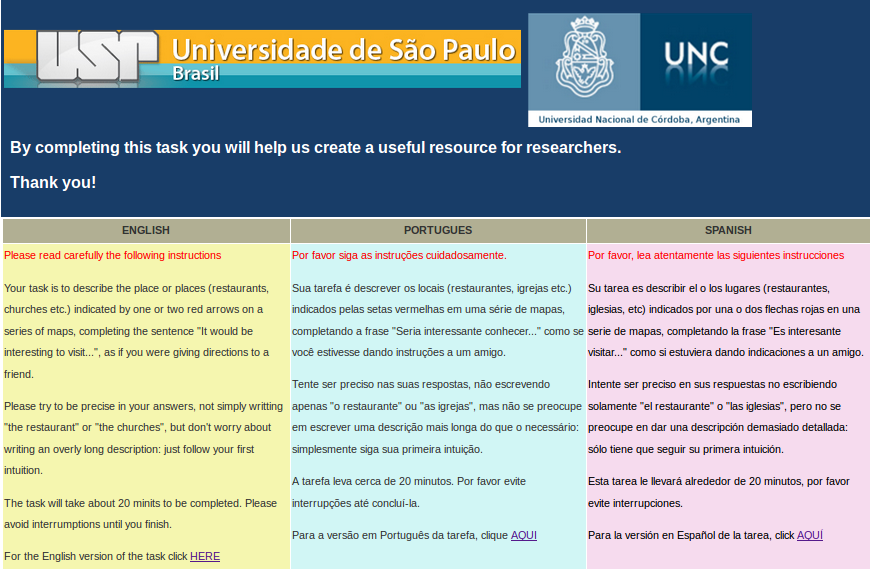
\includegraphics[width=13cm]{images/pagPrincipal.png}\\[0pt]
\caption{Link del experimento}
\label{fig-pagPrincipal}
\end{center}
\end{figure}

\begin{figure}[ht]
\begin{center}
\frame{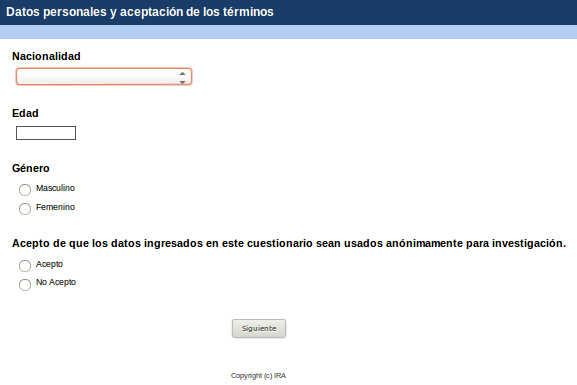
\includegraphics[width=13cm]{images/nacionalidadGenero.png}}\\[0pt]
\caption{Datos requeridos}
\label{fig-nacionalidadGenero}
\end{center}
\end{figure}

\begin{figure}[ht]
\begin{center}
\frame{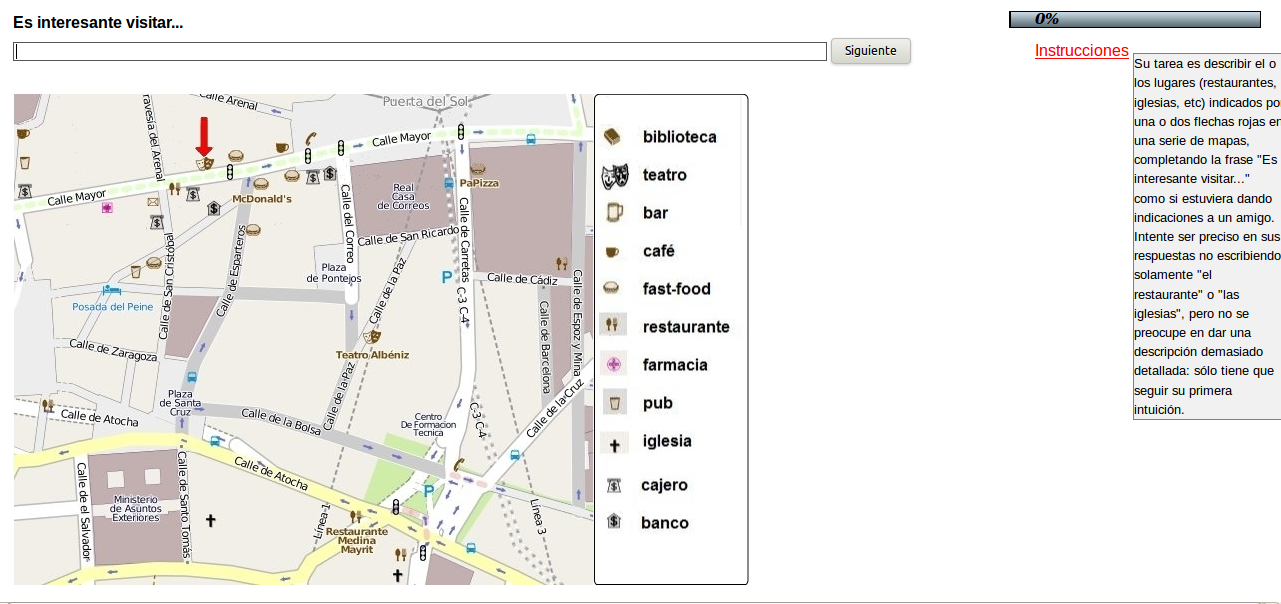
\includegraphics[width=15cm]{images/primerImagen.png}}\\[0pt]
\caption{Interface del experimento}
\label{fig-interface}
\end{center}
\end{figure}




